% !TeX spellcheck = en_GB
\section{Operational weather forecast model - MEPS}\label{sec:DIM:MEPS}
MEPS (MetCoOp Ensemble Prediction System) was newly operational at Met-Norway when the extreme weather occurred in Norway. Comparing model data with actual observations helps to verify the agreement between model prediction and ground-based measurements. 
\\
AROME-MetCoOp was operational from March 2014 until November 2016, when it was replaced with an ensemble prediction system (EPS) based on AROME-MetCoOp.
MEPS is used as weather forecast at the Norwegian Meteorological Institute, the Swedish Meteorological and Hydrological Institute (SMHI) and the Finnish Meteorological Institute (FMI), \citep{muller_arome-metcoop:_2017, koltzow_metcoop_2017}.
\\
\\
%Ensemble prediction has the goal to improve the forecast by ensemble averaging, to provide an indication of the reliability of the forecast, and a quantitative basis for probabilistic forecasting \citep{kalnay_atmospheric_2003}. 
\textcolor{red}{Include the difference between AROME-MetCoOp and MEPS \\
  } %Ein ensemble Vorhersagesystem erfordert die Definition der Anfangsamplitude und die horizontal eun vertikale Struktur der Störung. In der Regel wird die Anfangs Amplitude so gewählt, dass sie nahe an den Beobachtungen liegth. Die Anfangsbedingung für die Störung liegt innerhalb eines Kreises (abbildung) der Beobachtungsunsicherheit. In der Regel liegen die Vorhersagen nahe beieinander für den kurzen Vorhersagebereich und können als deterministisch betrachtet werden. Nach einer bestimmten zeit sind die Prognosen der unterschiedlichen Störugsmitglieder so groß, dass sie als stochastisch betrachtet werden müssen. Für die Vorhersage von großräumigen Störungen liegt die Übergangszeit in der Größenordnung von zwei bis drei Tagen. Für die Vorhersage von mesoskaligen Phänomenen kann dies nur wenige Stunden betragen.
%\\
%Der Unterschied zwischen AROME-MetCoOp und MEPS liegt darin, dass AROME-MetCoOp nur eine deterministische Vorhersage enthält, wobei MEPS neun weitere Störungsmitglieder der deterministischen Vorhersage besitzt.
%%%%%%%%%%%%%%%%%%%%%%%%%%%%%%%%%%%%%%%%%%%%%%%%%%%%%%%%%%%%%%%%%%%%%%%%%%
%%%%%%%%%%%%%%%%%%%%%%%%%%%%%%%%%%%%%%%%%%%%%%%%%%%%%%%%%%%%%%%%%%%%%%%%%%
%%%%%%%%% MEPS %%%%%%%%%%%%%%
\subsection{MetCoOP Ensemble Prediction System - MEPS}
In principle, MEPS is a short-term weather forecast consisting of a ten ensemble member  forecast system with \SI{66}{\hour} prediction time and a horizontal resolution of \SI{2.5}{\km} and 65 vertical levels. One of the members is the deterministic forecast where the other nine present the perturbed state of the deterministic forecast. The initialisation of each member is performed at \SIlist{00;06;12;18}{\UTC} \citep{metcoop_wiki_description_2017}.
\\ 
Forecast data saved for the deterministic and first ensemble member have a time resolution of one hour for \SI{66}{\hour}. The other eight members have values every three hours for up to \SI{48}{\hour} forecast time.
%\\
%%% image MEPS resolution %%%%%%%%%%%%%%%%%%%%%%%%%%%%%%%%%%%%%
% !TeX spellcheck = en_GB
% \begin{figure}[t]
% 	\centering
%     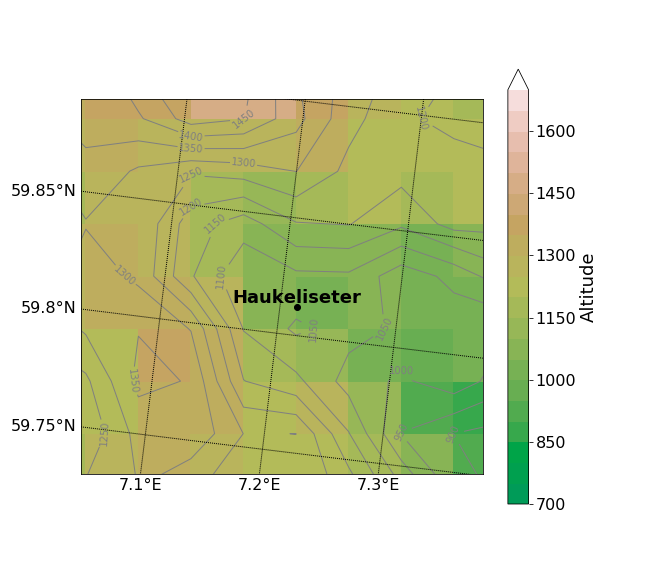
\includegraphics[trim={.3cm 2.2cm 1.8cm 2.4cm},clip,width=\textwidth]{./fig_Norway/MEPS_elevation_Haukeli}
%         \caption{}\label{fig:meps:site}
% \end{figure}

% \begin{wrapfigure}[14]{r}{0.55\textwidth}
% 	\vspace{-\normalbaselineskip}
% 	\centering
% 	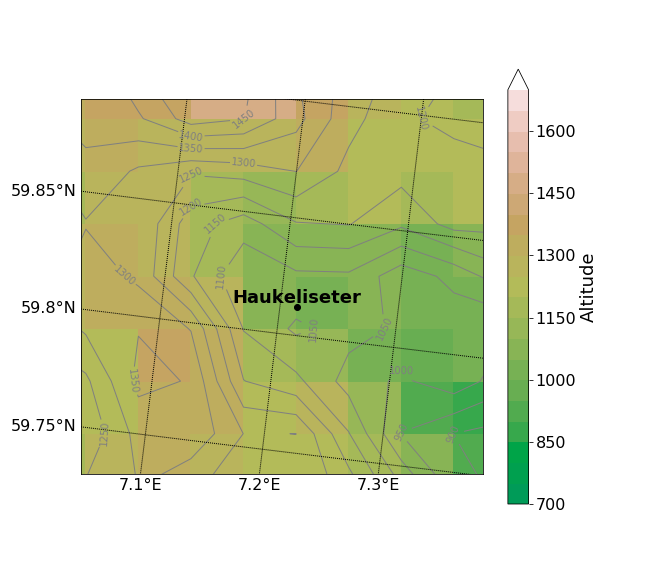
\includegraphics[trim={.3cm 2.2cm 1.8cm 2.4cm},clip,width=0.54\textwidth]{./fig_Norway/MEPS_elevation_Haukeli}
% 	%	\vspace{-10pt}
% 	\caption{Representation of the topography around measurement site Haukeliseter in MEPS. Contours and shading present the elevation of the grid cells.}\label{fig:meps:site}
% 	\vspace{-\normalbaselineskip}
% \end{wrapfigure}

% !TeX spellcheck = en_GB
\begin{figure}[ht!]
	\centering
    \begin{subfigure}[b]{0.53\textwidth}
    	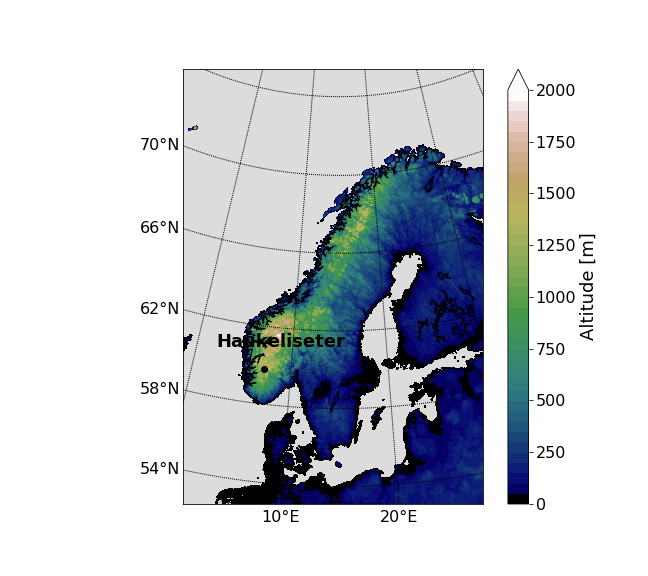
\includegraphics[trim={4.cm 1.8cm 0cm 2.cm},clip,width=1.05\textwidth]{./fig_Norway/Norway_elevation_MEPS}
        \caption{}\label{fig:meps:Norway}
    \end{subfigure}
    \begin{subfigure}[b]{0.46\textwidth}
        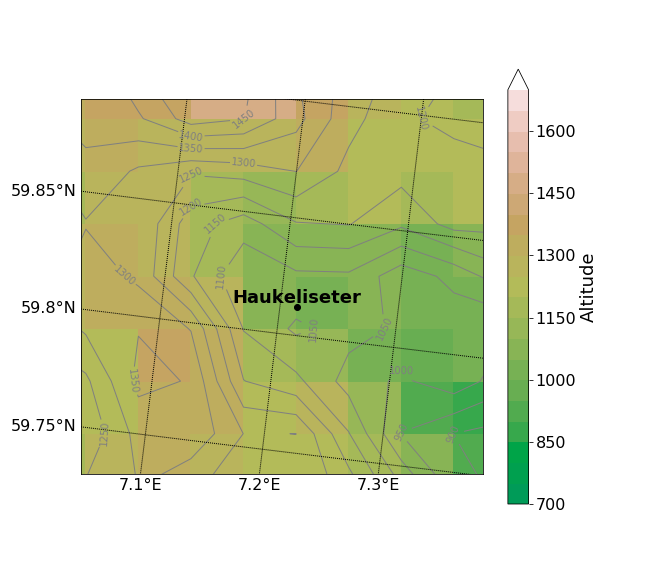
\includegraphics[trim={.3cm 2.2cm 1.8cm 2.4cm},clip,width=\textwidth]{./fig_Norway/MEPS_elevation_Haukeli}
        \caption{}\label{fig:meps:site}
      \end{subfigure}
	\caption{\protect\subref{fig:meps:Norway}: Elevation map of MEPS model domain. \protect\subref{fig:meps:site}: Representation of the topography around the measurement site Haukeliseter in MEPS. Contours and shading present the elevation of the grid cells.}\label{fig:meps_site}
\end{figure} 
%%%%%%%%%%%%%%%%%%%%%%%%%%%%%%%%%%%%%%%%%%%%%%%%%%%%%%%%%%%%%%%%%%%%%%%%%%
\noindent
\Cref{fig:site:Norway} shows the MEPS model domain and its elevation as it was operational for December 2016. It covers the Nordic Countries including open water such as the Atlantic Ocean, the North and the Baltic Sea. A representation of the horizontal resolution zoomed on the Haukeliseter site is shown in \Cref{fig:meps:site}. Haukeliseter is surrounded by a complex terrain with mountains up to \SI{1500}{\metre} no the west and the north and the more open terrain to the south-east.
\\
The centre of the model is approximately at \ang{63.5}\,N, \ang{15}\,E. 
The horizontal grid points are projected on a Lambert projection to receive the same area size of each grid cell. 
%The outer, parent grid is the ECMWF-IFS model (European Centre for Medium-Range Weather Forecasts Integrated Forecasting System) with a horizontal resolution of \SI{9}{\km} \citep{homleid_verification_2016}. The ECMWF-IFS forecasts are used \SI{6}{\hour} prior to the actual cycle in MEPS.
The regional model MEPS receives initial and boundary conditions from ECMWF-IFS (European Centre for Medium-Range Weather Forecasts Integrated Forecasting System) before it can produce forecasts \citep{muller_arome-metcoop:_2017}. The horizontal resolution of the parent ECMWF grid is \SI{9}{\km} \citep{homleid_verification_2016}. The ECMWF-IFS forecasts are used \SI{6}{\hour} prior to the actual cycle in MEPS.
Since initial conditions such as observations have uncertainties as well as the model has mistrust, and  the own climatology needs to be approached, a model has to stabilize before the simulations can be trusted. The spin-up time varies depending on the quality of the initial and boundary conditions. 
\\
Vertical hybrid coordinates are terrain-following and are mass-based, \citep{muller_arome-metcoop:_2017}. How the vertical hybrid coordinates are transformed into layer thickness or height is described in \Cref{sec:layer_thickness}. Furthermore, MEPS underlies non-hydrostatic dynamics, \cite{metcoop_wiki_description_2017}.
\\
The representation of snow is covered by a modification of the three-class ice parametrization (ICE3) scheme. Where liquid-phase processes are separated from slow ice-phase processes and described in \Cref{sec:MesoNH}. To model the snow cover an one-layer atmosphere model scheme is implemented. This includes three variables such as: snow water equivalent (SWE), snow density, and snow albedo \citep{muller_arome-metcoop:_2017}.
\\
As synoptic observations are included in the model the snow-depth predictions underlay a special performance. Observations of snow-depth are only available at \SIlist{06;18}{\UTC}, therefore is the snow analysis only performed twice daily \citep{muller_arome-metcoop:_2017, homleid_verification_2016}. 
%The MEPS forecasting system consist of 1+9 members where each of the perturbed members perform an initialization of \SI{66}{\hour} at \SIlist{00;06;12;18}{\UTC} \citep{metcoop_wiki_description_2017}. 
%\\
%For more detailed information to the model the reader is referred to \cite{muller_arome-metcoop:_2017} and \cite{wiki_description_2017} and its references therein.
%
%%%%%%%%%%%%%%%%%%%%%%%%%%%%%%%%%%%%%%%%%%%%%%%%%%%%%%%%%%%%%%%%%%%%%%%%%%
%%%%%%%%%%%%%%%%%%%%%%%%%%%%%%%%%%%%%%%%%%%%%%%%%%%%%%%%%%%%%%%%%%%%%%%%%%
%%%%%%%%% MESONH %%%%%%%%%%%%%%
\subsection{Meso-NH and the ICE3 scheme} \label{sec:MesoNH}
The physical parametrization within AROME is based on the French research communities' mesoscale non-hydrostatic atmosphere model (Meso-NH). The microphysical scheme in the Meso-NH atmospheric simulation system is based on the ICE3 scheme. The purpose of the scheme is to model as correctly as possible the ice phase in the atmosphere \citep{pinty_mixed-phased_1998}. \cite{mccumber_comparison_1991} concluded from their case study, that at least three different ice categories are necessary to cover most precipitation but that applications might be case specific. 
According to the \cite{meteo_france_meso-nh_2009} documentation, the ice phase microphysical scheme must include: 
\begin{itemize}
	\item [\textbf{r$_i$:}] pristine ice phase  
	\item [\textbf{r$_s$:}] snowflake type from lightly rimed large ice crystals or dry clusters, and
	\item [\textbf{r$_g$:}] heavily rimed crystals, such as graupel, frozen drops or hail
\end{itemize}
% %%% table ice parameters %%%%%%%%%%%%%%%%%%%%%%%%%%%%%%%%%%%%%
% % % !TeX spellcheck = en_GB
\begin{table}[h]
	\begin{center}
		\caption{Characterization parameters from primary ice (r$_i$), snowflakes (r$_s$) and rimed crystals (r$_g$). Values are based on the references in \cite{meteo_france_meso-nh_2009} and in \cite{pinty_mixed-phased_1998}. }\label{tab:ice_parameter}
		\begin{tabular}{l|c|c|c}
			\hline \hline
			& \textbf{r$_i$}& \textbf{r$_s$}& \textbf{r$_g$} \\ \hline\hline
			$\alpha$, $\nu$ & \num{3.3}		& \num{1.1}			& \num{1.1} \\ \hline
			$a$				& \num{0.82}	& \num{0.02}		& \num{196} \\ 
			$b$				& \num{2.5}		& \num{1.9}			& \num{2.8} \\ \hline
			$c$				& \num{800}		& \num{5.1}			& \num{124} \\ 
			$d$				& \num{1.0}		& \num{0.27}		& \num{0.66} \\ \hline
			$C$				&				& \num{5}			& \num{5e5} \\
			$x$				&				& \num{1}			& \num{-0.5} \\
			\hline \hline
		\end{tabular}
	\end{center}
\end{table}
% %%%%%%%%%%%%%%%%%%%%%%%%%%%%%%%%%%%%%%%%%%%%%%%%%%%%%%%%%%%%%%%%%%%%%%%%%%
Within the ICE3 scheme no distinction between hail and graupel exists and therefore is the physical discrimination in the growth mode of graupel and hail is neglected. \\
To achieve snow water content within MEPS the total number concentration, slope parameter, mass diameter and  the particle size distribution have to be determined. 
According to \cite{caniaux_numerical_1994} follows the particle size distribution the Marshall-Palmer distribution similar to \Cref{eq:num_dens}. The goal is to use a varying number concentration $N_0$ dependent on the ice category. The study has shown that $N_0$ can be assumed with
\begin{align}
	N_0 & = C \lambda^x  \label{eq:model_N0}
	\\
	\log_{10}C & = -3.55x + 3.89  \nonumber
\end{align}
where $C$ and $x$ depend on the ice category and represent the relation between each other in \Cref{eq:model_N0}. 
\\
The ice water content for primary ice, snowflakes and rimed crystals is then be assumed to be similar to \Cref{eq:SWC}, but the integration limits range from zero to infinity and mass, and particle size distribution are dependent on the diameter of the particle. The mass diameter and particle size distribution (\Cref{eq:mass_diameter,eq:PSD_MEPS}) are represented depending on the ice category shown in \Cref{tab:ice_parameter}
\begin{align}
	m(D) & = aD^b 	\label{eq:mass_diameter} \\
	n(D) & = N_0 g(D)	\label{eq:PSD_MEPS}
\end{align}
and $g(D)$ to be the generalised Gamma function 
\begin{align}
	g(D) = \frac{\alpha}{\Gamma(\nu)} \lambda^{\alpha \nu} D^{\alpha \nu -1} \exp\left( -(\lambda D)^\alpha \right)
\end{align}
with $\alpha$, $\nu$ the shape and tail dispersion parameters and $\Gamma(\nu)$ the gamma function. 
\\
After following the above equations including \Cref{eq:SWC} the slope parameter $\lambda$ can be generated with $G(B)$ the gamma function.
\begin{align}
	\lambda & = \left( \frac{\text{SWC}}{aCG(b)}\right)^{\frac{1}{x-b}}
\end{align}
%
%%% table ice parameters %%%%%%%%%%%%%%%%%%%%%%%%%%%%%%%%%%%%%
% % !TeX spellcheck = en_GB
\begin{table}[h]
	\begin{center}
		\caption{Characterization parameters from primary ice (r$_i$), snowflakes (r$_s$) and rimed crystals (r$_g$). Values are based on the references in \cite{meteo_france_meso-nh_2009} and in \cite{pinty_mixed-phased_1998}. }\label{tab:ice_parameter}
		\begin{tabular}{l|c|c|c}
			\hline \hline
			& \textbf{r$_i$}& \textbf{r$_s$}& \textbf{r$_g$} \\ \hline\hline
			$\alpha$, $\nu$ & \num{3.3}		& \num{1.1}			& \num{1.1} \\ \hline
			$a$				& \num{0.82}	& \num{0.02}		& \num{196} \\ 
			$b$				& \num{2.5}		& \num{1.9}			& \num{2.8} \\ \hline
			$c$				& \num{800}		& \num{5.1}			& \num{124} \\ 
			$d$				& \num{1.0}		& \num{0.27}		& \num{0.66} \\ \hline
			$C$				&				& \num{5}			& \num{5e5} \\
			$x$				&				& \num{1}			& \num{-0.5} \\
			\hline \hline
		\end{tabular}
	\end{center}
\end{table}
%%%%%%%%%%%%%%%%%%%%%%%%%%%%%%%%%%%%%%%%%%%%%%%%%%%%%%%%%%%%%%%%%%%%%%%%%%
%
%%% image ICE3 scheme  %%%%%%%%%%%%%%%%%%%%%%%%%%%%%%%%%%%%%
% !TeX spellcheck = en_GB
\begin{figure}[h]
	\centering
	%    \begin{subfigure}[b]{\textwidth}
	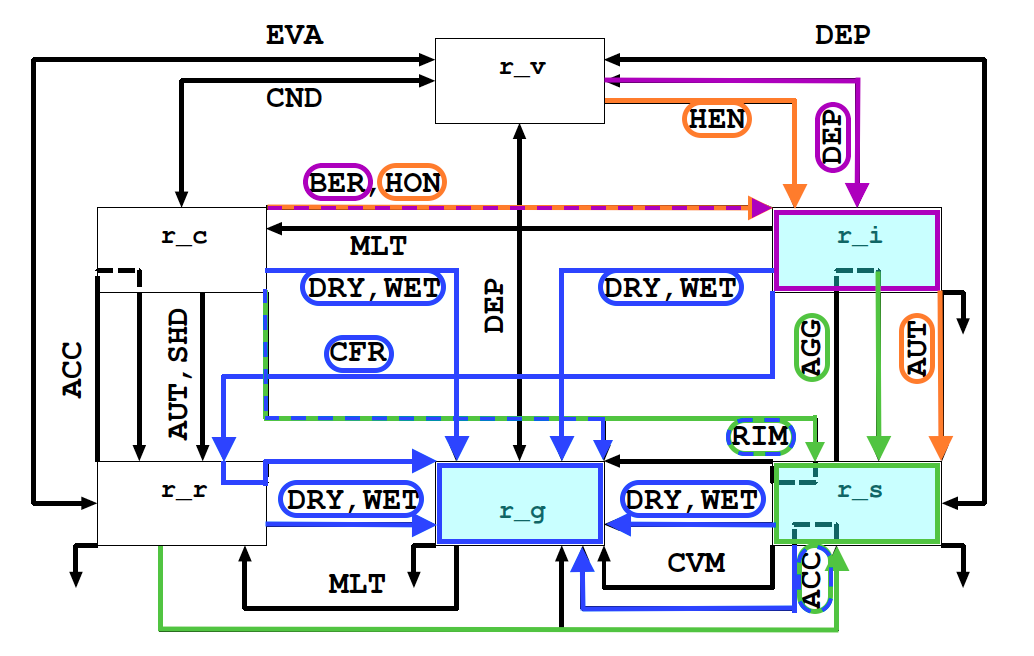
\includegraphics[width=\textwidth]{./fig_MEPS/ICE3_scheme_copy}
	%	\end{subfigure}
	\caption{Microphysical processes for mixed phase clouds in the ICE3 scheme adapted from \cite{meteo_france_meso-nh_2009}. In orange the initiation processes for primary ice r$_i$ and snowflakes r$_s$. The growing processes of r$_i$ is shown in purple and for r$_s$ in green. Graupel particles, r$_g$, grow from existent particles and the processes are shown in blue. }\label{fig:ICE3_scheme}
\end{figure}
%%%%%%%%%%%%%%%%%%%%%%%%%%%%%%%%%%%%%%%%%%%%%%%%%%%%%%%%%%%%%%%%%%%%%%%%%%
\newline
\cite{meteo_france_meso-nh_2009} documentation suggests starting the microphysics in the ICE3 scheme with 'slow' processes such as homogeneous and heterogeneous nucleation (HON, HEN), vapour deposition of snow and graupel particles (DEP), aggregation (AGG) and auto conversion (AUT), for ice processes right side in \Cref{fig:ICE3_scheme}. The second step is to initiate the warm processes left side in \Cref{fig:ICE3_scheme}. Then include the aggregation and conversion-melting (CVM) for snowflakes and contact freezing of raindrops (CFR). Add AGG and melting for graupel (MLT), and then the melting from pristine ice  and the Wegener-Bergeron-Findeisen (BER) effect and lastly the sedimentation terms.  \\
\Cref{fig:ICE3_scheme} shows the summary of the microphysical processes for mixed phase clouds. The study focuses mostly on solid precipitation particles and therefore only the initiation and growth of pristine ice crystals r$_i$, snowflakes r$_s$, and rimed crystals r$_g$ is presented. 
\\
Following \cite{pinty_mixed-phased_1998} and \Cref{fig:ICE3_scheme} it can be seen how AROME performs the ice production. Orange lines in \Cref{fig:ICE3_scheme} show the initiation of pristine ice crystals and snowflakes. In purple the growth mechanisms of r$_i$ (BER,DEP). Green lines demonstrate the expansion of the snowflakes (RIM, AGG, ACC). Graupel (r$_g$) forms as an effect of heavy riming (RIM), by collision of larger raindrops with snowflakes (ACC), by WET/DRY growth or by contact freezing of raindrops (CFR). All graupel growth processes are indicated by blue lines in \Cref{fig:ICE3_scheme}, were hail formation is included. 

% are the primary ice crystals activated by either heterogeneous nucleation (HEN), when some ice nuclei are present or by homogeneous nucleation (HON), when the atmospheric temperature is below \SI{-35}{\celsius}. The growing process for these particles can be the Bergeron-Findeisen process (BER) or deposition of water vapour (DEP). \\
% Snow particles are initiated by auto conversion (AUT) of r$_i$ and grow by the riming of cloud droplets (RIM) or rain droplets (ACC), and by collection of small pristine crystals (AGG), indicated by the green lines in \Cref{fig:ICE3_scheme}. \\
% As indicated by the blue lines in \Cref{fig:ICE3_scheme} are graupel an effect of heavy riming and grow in the scheme if the riming aggregates are of larger diameter size than \SI{7}{\mm} \citep{meteo_france_meso-nh_2009}. As indicated can graupel also grow when larger colliding raindrops reshape snowflakes to graupel (ACC). Furthermore, is graupel growth affected by wet or dry (WET, DRY) accretion, when the surface temperature of graupel is larger than the environmental temperature. DRY graupel expansion happens as long as the surface temperature is less that the surrounding temperature, then collected drops will freeze. WET graupel growth appears, when a liquid film is on the surface of the graupel particle (surface temperature larger than surrounding) then the liquid condensate is shed away, and hail will be formed. In ICE3 is hail not specifically included it is mixed in to the graupel category and therefore a distinction between the two categories cannot be made. 

%
\subsection{Adjustment of ICE3 inside AROME-MetCoOp}
% refinement for AROME 
Since the ICE3 scheme showed some weaknesses for the winter month, \cite{muller_arome-metcoop:_2017} introduced some modifications. 
During cold conditions the ICE3-scheme showed too low temperature at two meter, too much ice fog and all year long was the occurrence of cirrus overestimated. After implementing the modifications described in \cite{muller_arome-metcoop:_2017} the two meter temperature bias was reduced as well as an improvement of low-level clouds was shown. A negative aspect of these adjustments was that the occurrence of fog increased.%, by an error in the surface scheme.

% %%%%%%%%%%%%%%%%%%%%%%%%%%%%%%%%%%%%%%%%%%%%%%%%%%%%%%%%%%%%%%%%%%%%%%%%%%
% %%%%%%%%%%%%%%%%%%%%%%%%%%%%%%%%%%%%%%%%%%%%%%%%%%%%%%%%%%%%%%%%%%%%%%%%%%
% %%%%%%%%% SURFEX %%%%%%%%%%%%%%
% \section{SURFEX}
% \cite{masson_surfexv7.2_2013} \\
% SURFEX stands for 'surface externalisée' and is introduced into NWP models to ensure the consistent treatment of surface processes. It simulates the exchange of energy between four surface types and the atmosphere \citep{homleid_verification_2016}.

%%%%%%%%%%%%%%%%%%%%%%%%%%%%%%%%%%%%%%%%%%%%%%%%%%%%%%%%%%%%%%%%%%%%%%%%%%
%%%%%%%%%%%%%%%%%%%%%%%%%%%%%%%%%%%%%%%%%%%%%%%%%%%%%%%%%%%%%%%%%%%%%%%%%%












